\section{Amortized $O(1)$ Latent Plan Distillation (\texttt{DistilledJAXPlanner})}

While graph planning successfully avoids dead-ends, maintaining an offline graph and executing shortest-path queries introduces runtime overhead and memory footprint. To eliminate online graph lookups entirely, we formulate \textbf{Amortized Latent Plan Distillation}: compressing the topological knowledge of the Dijkstra teacher into an $O(1)$ feedforward neural student $\text{Student}_\theta(s_t, B(g)) \to \hat{z}_{\text{cmd}}$ that directly drives the low-level policy $\pi^\ell$.

\begin{figure}[t]
    \centering
    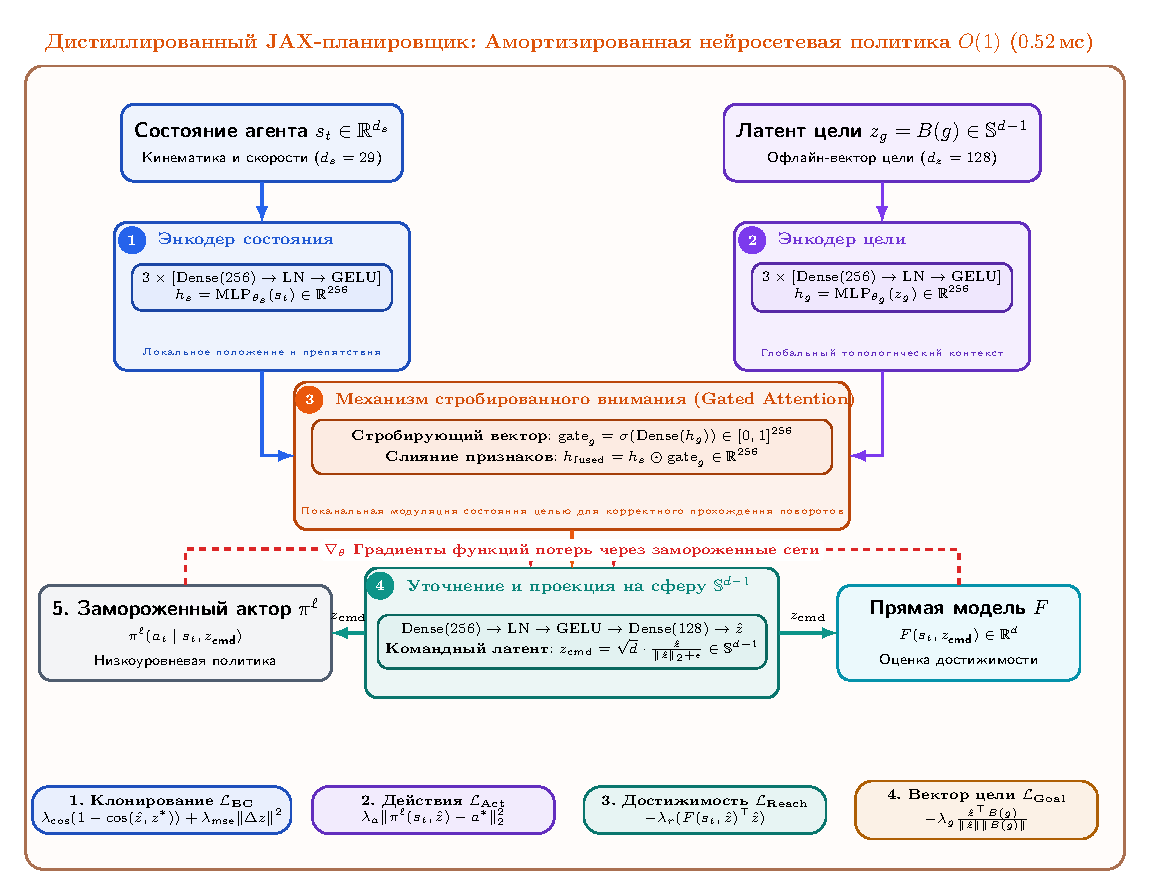
\includegraphics[width=\linewidth]{figures/fig3_distilled_jax.pdf}
    \caption{\textbf{Amortized JAX Gated-Attention Distillation}: The student network $\text{Student}_\theta(s_t, B(g))$ predicts the intention vector $\hat{z}$ directly on the unit sphere $\mathbb{S}^{d-1}$ and is trained end-to-end using an automatic differentiable 4-component physics-grounded loss.}
    \label{fig:distilled_jax}
\end{figure}

\subsection{Architectures Explored}
We evaluated multiple neural student architectures for amortized planning:
\begin{enumerate}[leftmargin=*,noitemsep]
    \item \textbf{Standard MLP with LayerNorm (\texttt{mlp})}: 4-layer perceptron with GELU activations and spherical projection.
    \item \textbf{Dense Residual Network with Efficient Channel Attention (\texttt{dense\_eca})}: Dense skip connections across all intermediate representations with 1D adaptive channel attention.
    \item \textbf{Gated Cross-Attention Network (\texttt{gated\_attn})}: Distinct state and goal encoders where goal features query state representations via Multi-Head Cross-Attention, followed by sigmoid gating:
    \begin{align}
        h_s &= \text{MLP}_s(s_t), \quad h_g = \text{MLP}_g(B(g)) \\
        h_{\text{cross}} &= \text{CrossAttention}(Q = h_g, K = h_s, V = h_s) \\
        \gamma &= \sigma(\text{Linear}([h_s, h_{\text{cross}}])) \\
        h_{\text{fused}} &= \gamma \odot h_{\text{cross}} + (1 - \gamma) \odot h_s \\
        \hat{z}_{\text{cmd}} &= \sqrt{d} \cdot \frac{\text{Head}(h_{\text{fused}})}{\|\text{Head}(h_{\text{fused}})\|_2}
    \end{align}
\end{enumerate}

\subsection{Differentiable 4-Component Physics Loss Formulation}
Rather than training via naive mean squared error on latent vectors, we formulate a multi-objective loss that differentiates directly through the frozen low-level policy $\pi^\ell$ and the frozen forward representation $F(s, z)$:
\begin{equation}
    \mathcal{L}(\theta) = \mathcal{L}_{\text{BC}}(\hat{z}, z^*) + \lambda_1 \mathcal{L}_{\text{Action}}(\hat{z}) + \lambda_2 \mathcal{L}_{\text{Reach}}(\hat{z}) + \lambda_3 \mathcal{L}_{\text{Goal}}(\hat{z})
    \label{eq:distill_loss}
\end{equation}
where:
\begin{align}
    \mathcal{L}_{\text{BC}}(\hat{z}, z^*) &= (1 - \cos(\hat{z}, z^*)) + \frac{1}{d}\|\hat{z} - z^*\|_2^2 \\
    \mathcal{L}_{\text{Action}}(\hat{z}) &= \|\pi^\ell(s_t, \hat{z}) - a^*_{\text{teacher}}\|_2^2 \\
    \mathcal{L}_{\text{Reach}}(\hat{z}) &= - \left(F(s_t, \hat{z})^\top \hat{z}\right) \\
    \mathcal{L}_{\text{Goal}}(\hat{z}) &= - \left(\hat{z}^\top B(g)\right)
\end{align}

\begin{keyinsight}[Physics Grounding via Frozen $\pi^\ell$ and $F$]
The term $\mathcal{L}_{\text{Action}}$ penalizes predictions $\hat{z}$ that would cause the low-level policy $\pi^\ell$ to produce conflicting torques, while $\mathcal{L}_{\text{Reach}}$ encourages $\hat{z}$ to lie in high-reachability manifolds of the forward model $F(s, \hat{z})$. Thanks to JAX automatic differentiation (\texttt{jax.value\_and\_grad}), gradients $\nabla_\theta \mathcal{L}$ flow seamlessly through the complex neural layers of frozen $\pi^\ell$ and $F$ without approximations.
\end{keyinsight}
